% !TEX root = ../../../main.tex
% 来源：高中物理甲种本·第三册（电磁·光学·近代物理）
% 章节：交流电 / 三相电路的连接
% 原始文件：3.tex，行 1741-1765
% 类型：tikz
% ---
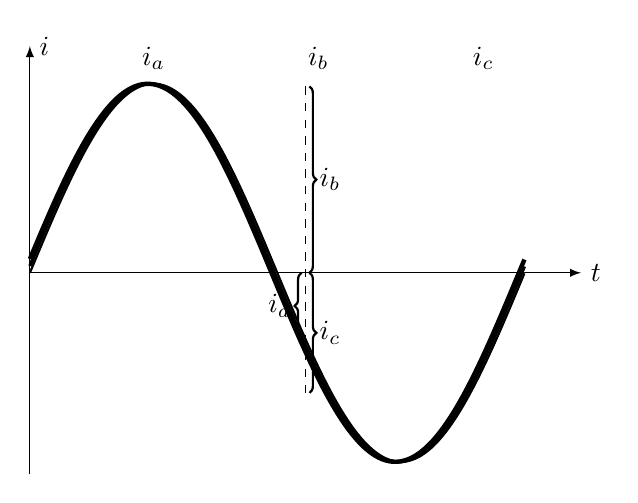
\begin{tikzpicture}[>=latex, yscale=1.6]
    %\draw [|<->|](3.7,1.4796)--node[fill=white]{$i_b$}(3.7,0);
%\draw [|<->|](3.3,-0.9534)--node[fill=white]{$i_c$}(3.3,0);
%\draw [|<->|](3.7,-.5262)--node[fill=white]{$i_a$}(3.7,0);

\draw[decorate,decoration=brace, thick](3.55,1.4796)--node[right]{$i_b$}(3.55,0);
\draw[decorate,decoration=brace, thick](3.55,0)--node[right]{$i_c$}(3.55,-0.9534);
\draw[decorate,decoration=brace, thick](3.45,-.5262)--node[left]{$i_a$}(3.45,0);


\draw[->] (0,-1.6)--(0,1.8)node [right]{$i$};
\draw [->](0,0)--(7,0)node [right]{$t$};
\draw [thick] plot [domain=0:3.1416*2, samples=1000, variable=\x] (\x, {1.5*sin(\x r)}) ;
\draw [very thick] plot [domain=0:3.1416*2, samples=1000, variable=\x] (\x, {1.5*sin(3.1416*2/3+\x r)}) ;
\draw [ultra thick] plot [domain=0:3.1416*2, samples=1000, variable=\x] (\x, {1.5*sin(3.1416*4/3+\x r)}) ;
\node at (3.1416/2, 1.7){$i_a$};
\node at (3.1416/2+3.1416*2/3, 1.7){$i_b$};
\node at (3.1416/2+3.1416*4/3, 1.7){$i_c$};



\draw[dashed](3.5, 1.4796)--(3.5,-0.9534);


\end{tikzpicture}
